%  LaTeX support: latex@mdpi.com 
%  In case you need support, please attach all files 
%  that are necessary for compiling as well as the log file, 
%  and specify the details of your LaTeX setup 
%  (which operating system and LaTeX version / tools you are using).

%=================================================================
\documentclass[ijgi,article,submit,moreauthors,pdftex]{Definitions/mdpi} 


%=================================================================
\firstpage{1} 
\makeatletter 
\setcounter{page}{\@firstpage} 
\makeatother
\pubvolume{xx}
\issuenum{1}
\articlenumber{5}
\pubyear{2019}
\copyrightyear{2019}
%\externaleditor{Academic Editor: name}
\history{Received: date; Accepted: date; Published: date}
%\updates{yes} % If there is an update available, un-comment this line

%% MDPI internal command: uncomment if new journal that already uses continuous page numbers 
%\continuouspages{yes}

%------------------------------------------------------------------
% The following line should be uncommented if the LaTeX file is uploaded to arXiv.org
%\pdfoutput=1

%=================================================================
% Add packages and commands here. The following packages are loaded in our class file: fontenc, calc, indentfirst, fancyhdr, graphicx, lastpage, ifthen, lineno, float, amsmath, setspace, enumitem, mathpazo, booktabs, titlesec, etoolbox, amsthm, hyphenat, natbib, hyperref, footmisc, geometry, caption, url, mdframed, tabto, soul, multirow, microtype, tikz

\usepackage{xspace}
\usepackage{mathtools}
\usepackage{fancyvrb} %for \begin{Verbatim} environment; color in verbatime



\usepackage{xcolor,listings}
\usepackage{textcomp}
\lstset{upquote=true}






%\usepackage[T1]{fontenc}
%\usepackage{subcaption}
%=================================================================
%% Please use the following mathematics environments: Theorem, Lemma, Corollary, Proposition, Characterization, Property, Problem, Example, ExamplesandDefinitions, Hypothesis, Remark, Definition, Notation, Assumption
%% For proofs, please use the proof environment (the amsthm package is loaded by the MDPI class).

%so that we have more tolerance for large figures
%large figure is less likely to push to the end of the document
\renewcommand{\textfraction}{0.01}
\renewcommand{\topfraction}{0.99}
\renewcommand{\bottomfraction}{0.99}
\renewcommand{\dbltopfraction}{0.99} % fit big float above 2-col. text

\graphicspath{{images/}}

\newcommand{\astar}{A$^{\!\star}$\xspace}

\newcommand{\e}[1]{\times 10^{#1}}
\newcommand{\fig}{Figure~}
\newcommand{\eq}{Equation~}
\newcommand{\fo}{Formula~}
\newcommand{\sect}{Section~}
\newcommand{\tbl}{Table~}
\newcommand{\chap}{Chapter~}
\newcommand{\figs}{Figures~}
\newcommand{\eqs}{Equations~}
\newcommand{\fos}{Formulas~}
\newcommand{\sects}{Sections~}
\newcommand{\tbls}{Tables~}
\newcommand{\chaps}{Chapters~}
\newcommand{\eg}{e.g.,~}
\newcommand{\ie}{i.e.,~}
\newcommand{\p}{p.~}
\newcommand{\pp}{pp.~}

\makeatletter
\def\verbatim@font{\normalfont\rmfamily}
\makeatother


%=================================================================
% Full title of the paper (Capitalized)
\Title{An Approach to Evaluating Merging Sequences}
%\Title{Merging land-cover areas parallelly 
%to support smooth zooming of web maps}

% Author Orchid ID: enter ID or remove command
\newcommand{\orcidauthorA}{0000-0000-000-000X} % Add \orcidA{} behind the author's name
%\newcommand{\orcidauthorB}{0000-0000-000-000X} % Add \orcidB{} behind the author's name

% Authors, for the paper (add full first names)
\Author{
Firstname Lastname $^{1,\dagger,\ddagger}$\orcidA{}, 
Firstname Lastname $^{1,\ddagger}$ and 
Firstname Lastname $^{2,}$*}

% Authors, for metadata in PDF
\AuthorNames{Firstname Lastname, Firstname Lastname and Firstname Lastname}

% Affiliations / Addresses (Add [1] after \address if there is only one affiliation.)
\address{%
$^{1}$ \quad Affiliation 1; e-mail@e-mail.com\\
$^{2}$ \quad Affiliation 2; e-mail@e-mail.com}

% Contact information of the corresponding author
\corres{Correspondence: e-mail@e-mail.com; Tel.: (optional; include country code; 
if there are multiple corresponding authors, add author initials) +xx-xxxx-xxx-xxxx (F.L.)}

% Current address and/or shared authorship
\firstnote{Current address: Affiliation 3} 
\secondnote{These authors contributed equally to this work.}
% The commands \thirdnote{} till \eighthnote{} are available for further notes

%\simplesumm{} % Simple summary

%\conference{} % An extended version of a conference paper

% Abstract (Do not insert blank lines, i.e. \\) 
\abstract{
When a map is zoomed out, some generalization operators are applied 
to simplify the map and to avoid visual clutter.
Merging is one of the frequently applied operators.
Many merging methods have been proposed.
This paper contributes to quantitatively evaluating 
sequences of merging land-cover areas.
We try to evaluate merging sequences obtained by a greedy algorithm
and an \astar algorithm in the aspects of class change and length change.
We implemented our evaluations in language PostgreSQL.
}

% Keywords
\keyword{PostgreSQL}



%%%%%%%%%%%%%%%%%%%%%%%%%%%%%%%%%%%%%%%%%%
% Only for the journal Data:
%\dataset{DOI number or link to the deposited data set in cases where the data set is published or set to be published separately. If the data set is submitted and will be published as a supplement to this paper in the journal Data, this field will be filled by the editors of the journal. In this case, please make sure to submit the data set as a supplement when entering your manuscript into our manuscript editorial system.}

%\datasetlicense{license under which the data set is made available (CC0, CC-BY, CC-BY-SA, CC-BY-NC, etc.)}



%\setcounter{secnumdepth}{4}
%%%%%%%%%%%%%%%%%%%%%%%%%%%%%%%%%%%%%%%%%%
\begin{document}
%%%%%%%%%%%%%%%%%%%%%%%%%%%%%%%%%%%%%%%%%%



\section{Introduction}





 
The existing methods evaluate a map at a certain scale.
This paper tries to evaluate a sequence of maps and the transitions.

The aim of this paper is to test some possible evaluation methods. 
The results do not suggest whether or not 
the algorithms of producing the merging sequences are good.
Those algorithm can be improved from many aspects.
 



Apparently, evaluating the changes for zooming is a new challenge,
which appear after dynamic maps are available.
\citet{Ruas2001Report} categorized some aspects of evaluating map generalization.
In the categorization are \emph{generalized data}, 
\emph{one generalization program}, \emph{one generalization program},
\emph{several generalization programs}, \emph{one generalization algorithms},
and \emph{generalization process(es)}.





 
%METHODS FOR EVALUATING THE RESULTS OF AUTOMATED GENERALIZATION 
%Formalization and data enrichment for automated evaluation of building pattern preservation 
%Methodology for evaluating automated map generalization in commercial software 
 
 
 
 
 
 
\section{Related Work}
\label{sec:realted_work}




\citet{Stoter2014Evaluation} gave a very good review 
of evaluation in map generalization.
\citet{Stoter2014Evaluation} pointed out 
an advantage and two disadvantages of evaluation.
The advantage is that 
the evaluation criteria help to improve the quality of map generalization.
A disadvantages is that 
the generalized result may violate some other criteria 
because the generalization process tries to fulfill the considered criteria.
The other disadvantage is that it may be impossible to evaluate 
the generalization results 
obtained from different systems \citep{Ruas2001Report}.
To overcome the problem in our case, 
we had to do some extra work.
The \astar algorithm was available in prototype
\emph{ContinuousGeneralizer}\footnote{Prototype ContinuousGeneralizer
    is open access on GitHub; 
	see	\url{https://github.com/IGNF/ContinuousGeneralisation}.}
We had to add a functionality 
to write the result of the \astar algorithm to a TXT file.
Then we read this file in prototype 
\emph{tgap}\footnote{Prototype tgap is open access on Bitbucket; 
	see	\url{https://bitbucket.org/bmmeijers/tgap}.}
and save the results as tables of tGAP tree in the PostgreSQL database
so that we can evaluate the result by a script written in 
PostgreSQL.






\citet{Ruas2001Report}

\citet{HaunertWolff2010AreaAgg}

\citet{Peng2017AStar}


%\section{Methodology}
%\label{sec:methodology}


\section{Evaluation}
\label{sec:evaluation}

%Regarding the persons who perform the evaluation, 
\citet{Ruas2001Report} mentioned an advantage and a disadvantage
when the persons who designed the system also perform the evaluation.
The advantage is the the persons know the details of the system well.
The disadvantage is that the persons may not be objective.
Fortunately, some of the authors of this paper 
participated in designing the greedy algorithm,
while the other authors were involved in developing the \astar algorithm.
Therefore, this paper can be objective to both algorithms.

Let $M_\mathrm{seq} = \{M_1, M_2, \dots, M_s, \dots\}$ be the map
at different states obtained from 
applying a sequence of merging operations.
Let $S_\mathrm{seq} = \{1, 2, \dots, s, \dots\}$ be the set of states.
For example, \fig\ref{fig:evaluations} has 
$M_\mathrm{seq} = \{M_1, M_2, M_3, M_4, M_5\}$ and
$S_\mathrm{seq} = \{1, 2, 3, 4, 5\}$.
%For the sake of convenience, we sometimes also refer to~$M_s$ as a map. 



\begin{figure*}[tb]
\centering
\includegraphics[page=2]{evaluations}
\caption{Some examples to illustrate how to compute the costs of an aggregation sequence.
}
\label{fig:evaluations}
\end{figure*}


\subsection{Class Change}



We have two preferences for the class change 
when generating intermediate states of the map.
First, the difference between an intermediate map and 
the previous map should be small 
(see \sect\ref{sec:class_change_previous}).
We have this preference because a smaller difference
will distract a user less.
Second, the difference between an intermediate map and the start map
should be small (see \sect\ref{sec:class_change_start}).
The preference is because we hope that the area classes of an intermediate map 
should be consistent with the start map as much as possible.
According to the preferences,
we define two cost functions, where the function returns a larger value
if the difference is bigger.

This paper considers only the merging operation.
Therefore, a generated map always has the same size as the start map.
The difference between two maps can be computed by
\begin{equation}
\label{eq:f_integral}
f_\mathrm{class} (s_i, s_j) = \int_{R_\mathrm{map}}
d_\mathrm{class}(c_i,c_j) da,
\end{equation}
where~$R_\mathrm{map}$ denotes the region of the map,
symbol~$da$ is the differential of the region,
variables~$c_i$ and~$c_j$ are respectively
the two classes of place~$da$ on the two maps, 
and function~$d_\mathrm{class}(c_i,c_j)$ 
returns the distance between the two classes.
\fig\ref{fig:evaluations_class_distance} shows an example of class distances.
%%%%%%%%%%%%%%%%%%%%%%%%%%%%
% distance --> cost ?
%%%%%%%%%%%%%%%%%%%%%%%%%%%%%%%%

\begin{figure*}[tb]
\centering
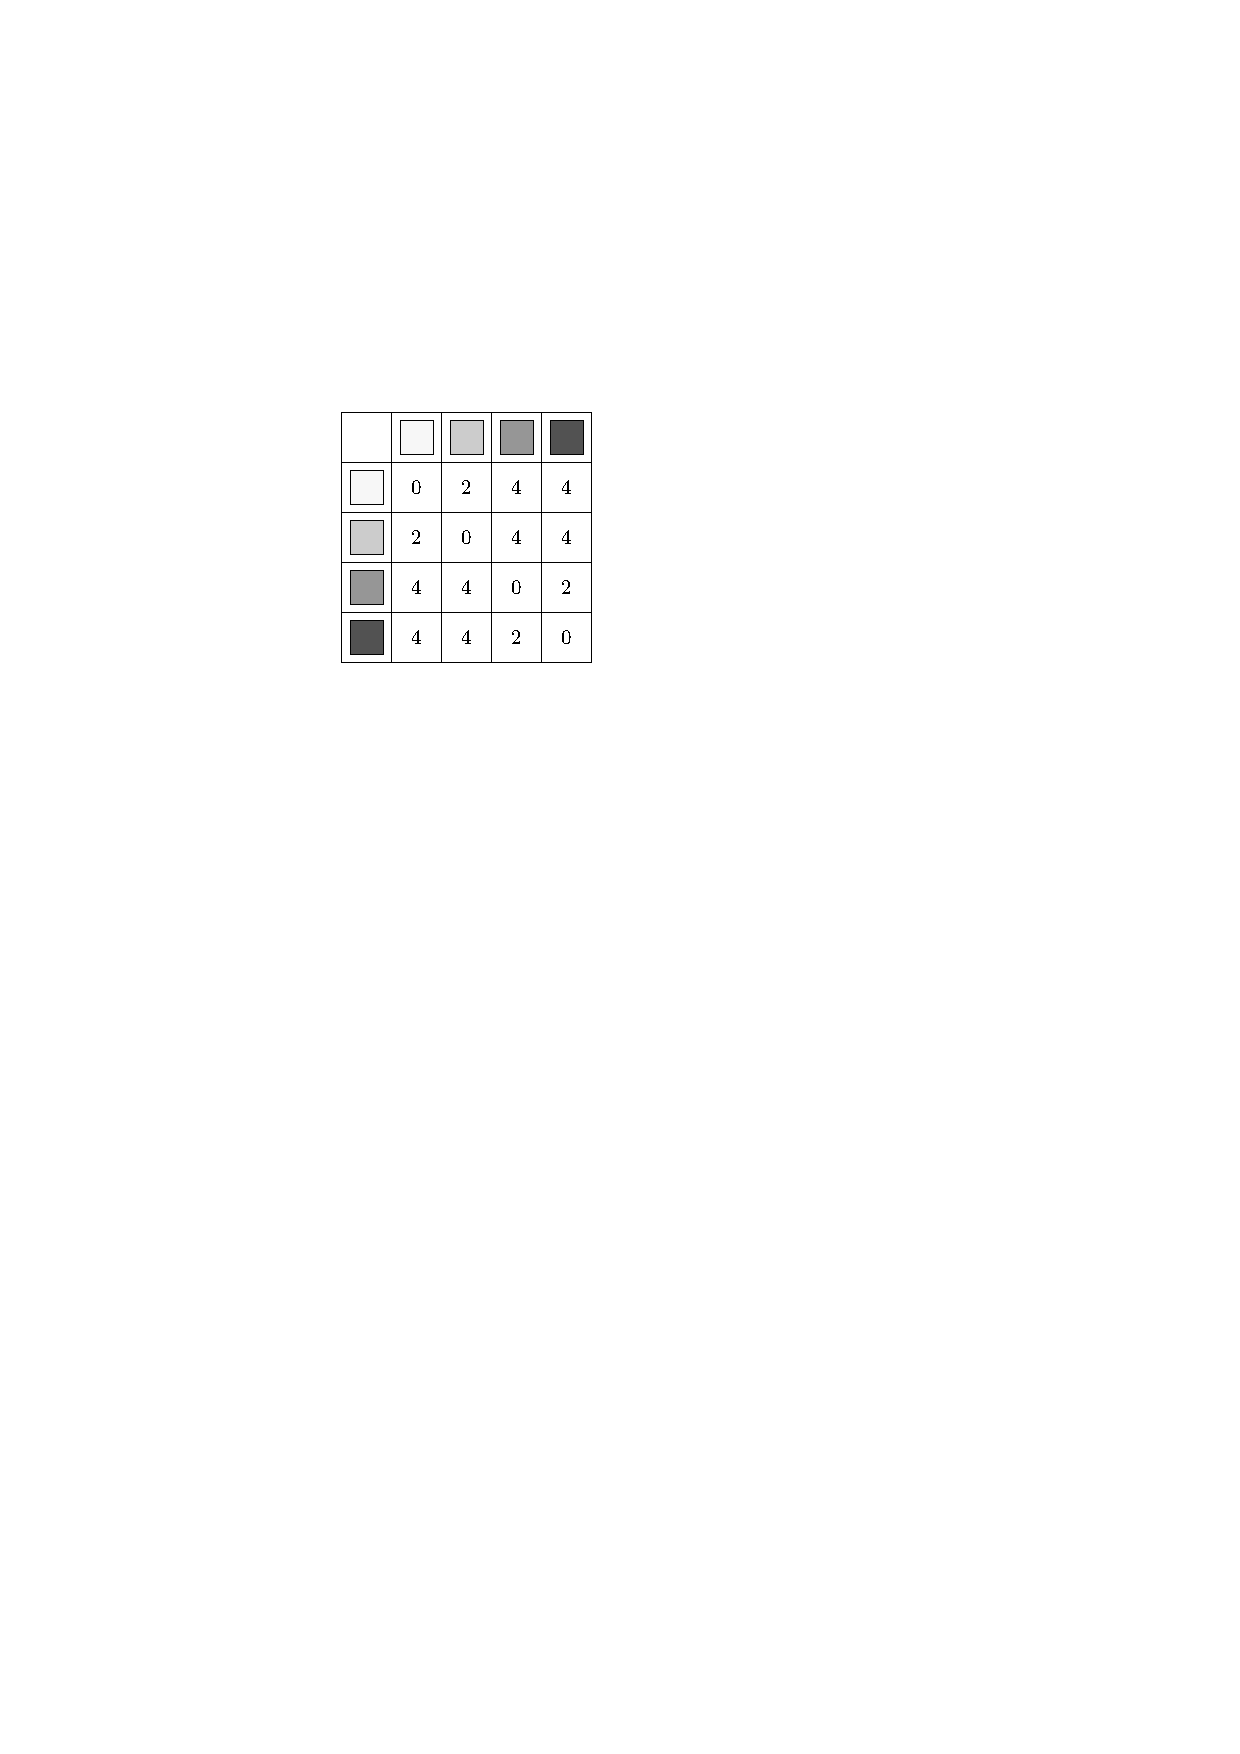
\includegraphics[page=1]{evaluations}
\caption{An example of class distances of land-cover areas, 
    where each color represents a class.
}
\label{fig:evaluations_class_distance}
\end{figure*}






\subsubsection{Class Change Against Previous State}
\label{sec:class_change_previous}

When we merge land-cover area~$p$ into land-cover area~$q$,
the class of~$p$ is changed to the class of~$q$.
Correspondingly, the map transits from state~$s-1$ to state~$s$.
Then \eq\ref{eq:f_integral} can be represented by
\begin{equation}
\label{eq:f_to_previous}
f_\mathrm{class}({s-1},s)=a_p \cdot d_\mathrm{class}(c(p),c(q)),
\end{equation}
%where variables~$M_{s-1}$ and~$M_s$ represent states~$s-1$ and~$s$ of a map.
where variable~$a_p$ is the size of land-cover area~$p$. 
Expressions~$c(p)$ and~$c(q)$ denote the classes of the two areas, respectively.
Formula~$d_\mathrm{class}(c(p),c(q))$ is the distance of the two classes.
The total cost of all the steps can be computed by
\begin{equation}
\label{eq:F_to_previous}
F_\mathrm{class} (S_\mathrm{seq}) =
\sum\limits_{i=2}^{|S_\mathrm{seq}|} f_\mathrm{class}(s_{i-1},s_i),
\end{equation}
where length~$|S_\mathrm{seq}|$ is the number of elements in set~$S_\mathrm{seq}$.

%If there are~$n$ land-cover areas on a map and 
%we merge 
%
%
%
%Take \fig\ref{fig:evaluations} for example, the corresponding areas of
%set~$C_{2,1}$ (the relevant places after  changing) and 
%set~$C_{1,2}$ (the relevant places before changing)
%should be similar in terms of land-cover classes.
%Therefore, we define the cost of class change of a step,
%from state~$s-1$ to state~$s$, as
%\begin{equation}
%\label{eq:F_class}
%F_\mathrm{class}(s)=\sum_{i=1}^{|C_{s-1,s}|} f_\mathrm{class}(p_i,q_i),
%\end{equation}
%where corresponding areas~$p_i$ and~$q_i$ are respectively from 
%the two sets of changed areas~$C_{s-1,s}$ and~$C_{s,s-1}$.
%There holds~$|C_{s-1,s}| = |C_{s,s-1}|$.
%According to the class distances defined in \fig\ref{fig:evaluations_class_distance},
%we have~$F_\mathrm{class}(2)=120$
%for class changes from set~$C_{1,2}$ to set~$C_{2,1}$ 
%(see \fig\ref{fig:evaluations}), and
%we have~$F_\mathrm{class}(3)=82$
%for class changes, from set~$C_{2,3}$ to set~$C_{3,2}$.

\subsubsection{Class Change Against Start Map}
\label{sec:class_change_start}
According to \eq\ref{eq:f_integral}, 
this cost can be obtained from computing~$f_\mathrm{class} (0, s)$.
That is, the difference between the map at state~$0$ (start map) and at state~$s$.
As we need to compute the total cost of a sequence of maps against the start map,
cost~$f_\mathrm{class} (0, s-1)$ should be computed before~$f_\mathrm{class} (0, s)$.
We reuse the already computed cost~$f_\mathrm{class} (0, s-1)$ 
to save some computation time.
In order to do so,
we need to define a function to compute the cost of 
an area against its components on start map.
For example, area~8 in \fig\ref{fig:evaluations} 
has areas~3, 4, and~5 as its components on the start map. 
Let~$r$ be the area, and let~$U$ be the set of components,
then we have cost
\begin{equation}
\label{eq:f_set}
g_\mathrm{class} (r) = 
\sum\limits_{u \in U} a_u \cdot d_\mathrm{class}(c(u),c(r)),
\end{equation}
where, similar to \eq\ref{eq:f_to_previous},
variable~$a_u$ is the size of land-cover area~$u$. 
Expressions~$c(u)$ and~$c(r)$ denote the classes of the two areas, respectively.


\begin{equation}
\label{eq:F_to_start}
f_\mathrm{class}(0,s)=f_\mathrm{class} (0, s-1) 
+ g_\mathrm{class} (r)
- g_\mathrm{class} (p)
- g_\mathrm{class} (q),
\end{equation}
where function~$f_\mathrm{class} (r)$ 
computes the cost of area~$r$'s class change against the start map.
Area~$r$ is the combination of a set of areas on the start map.




%We can take advantage of this  
%
%This computation can take advantage of~$f_\mathrm{class} (M_1, M_{s-1})$,
%which has already been computed.
%\begin{equation}
%\label{eq:F_to_start}
%f_\mathrm{class}(M_{s-1},M_s)=a_p \cdot d_\mathrm{class}(c(p),c(q)),
%\end{equation}

%Take \fig\ref{fig:evaluations} for example, the corresponding areas of
%set~$C_{3,1}$ (the relevant places after  changing) and 
%set~$C_{1,3}$ (the relevant places before changing)
%should be similar in terms of land-cover classes.
%We define this cost, from state~$1$ to state~$s$, as
%\begin{equation}
%\label{eq:F_class_prime}
%F'_\mathrm{class}(s)=\sum_{i=1}^{|C'_{1,s}|} f_\mathrm{class}(p'_i,q'_i),
%\end{equation}
%where corresponding areas~$p'_i$ and~$q'_i$ are respectively from 
%the two sets of changed areas~$C'_{1,s}$ and~$C'_{s,1}$.
%There holds~$|C'_{1,s}| = |C'_{s,1}|$.
%According to the class distances defined in \fig\ref{fig:evaluations_class_distance},
%we have~$F'_\mathrm{class}(3)=172$
%for class changes, from set~$C'_{1,3}$ to set~$C'_{3,1}$
%(see \fig\ref{fig:evaluations}).








\subsection{Length Change}

{\color{red}the length should not decrease evenly. 
Instead, it should decrease evenly on map.}

We also have two preferences for the shape when we generate intermediate maps.
First, the interior length should decrease evenly from the current map.
Take \fig\ref{fig:evaluations} for example, 
from state~$s=3$ the interior length should decrease by~$12$ at each step.
Therefore, we define the cost of length change of a step,
from state~$s-1$ to state~$s$, as
\begin{equation}
\label{eq:F_lgth}
F_\mathrm{lgth}(s)=
    \left(\ell_\mathrm{int}(s-1)-\ell_\mathrm{int}(s)-
        \frac{\ell_\mathrm{int}(s-1)}{n_\mathrm{state}-s+1}\right)^2,
\end{equation}
where expression~$\ell_\mathrm{int}(s-1)-\ell_\mathrm{int}(s)$ 
is the decrease of interior length from state~$s-1$ to state~$s$.
Parameter~$n_\mathrm{state}$ denotes the total number of states.
Expression~$\frac{\ell_\mathrm{int}(s-1)}{n_\mathrm{state}-s+1}$
is the average decrease of interior length from state~$s-1$ 
to a map with all the areas merged.
Take \fig\ref{fig:evaluations} for example,
we have~$n_\mathrm{state}=5$ and~$F_\mathrm{lgth}(3)=\frac{16}{9}$.


Our second preference of for the shape is that
the interior length should decrease evenly from the start map. 
Take \fig\ref{fig:evaluations} for example, 
from time~$state=1$ the interior length should decrease by~$11$ at each step.
We define this cost as
\begin{equation}
\label{eq:F_lgth_prime}
F'_\mathrm{lgth}(s)=
\left(\ell_\mathrm{int}(s-1)-\ell_\mathrm{int}(s)-
        \frac{\ell_\mathrm{int}(1)}{n_\mathrm{state}-1}\right)^2,
\end{equation}
where expression~$\frac{\ell_\mathrm{int}(1)}{n_\mathrm{step}-1}$
is the average decrease of interior length from state~$s=1$ 
to a map with all the areas merged.
Take \fig\ref{fig:evaluations} for example,
we have~$F'_\mathrm{lgth}(3)=1$.

We define the total cost of the whole aggregation sequence
based on \eqs\ref{eq:F_class}, \ref{eq:F_class_prime}, 
\ref{eq:F_lgth}, and \ref{eq:F_lgth_prime}. 
That is,
\begin{equation}
\label{eq:F}
F = \sum_{s=2}^{n_\mathrm{state}}
        \bigg(
            (2-\lambda)F_\mathrm{class}(s) +
            (2-\lambda)F'_\mathrm{class}(s) + 
            \lambda F_\mathrm{lgth}(s) +
            \lambda F'_\mathrm{lgth}(s)
        \bigg),
%F = \sum_{s=2}^{n_\mathrm{state}}
%        \left( 
%            (2-\lambda)F_\mathrm{class}(s) +
%            (2-\lambda)F'_\mathrm{class}(s) + 
%            \frac{\lambda d_\mathrm{class\_max}}{2} F_\mathrm{lgth}(s) +
%            \frac{\lambda d_\mathrm{class\_max}}{2}F'_\mathrm{lgth}(s)
%        \right),
\end{equation}
where parameter~$\lambda$ $(0\le \lambda \le 2)$ can be used to assign the importances of 
class change and length change.
In our experiment, we set $\lambda=1$.
%Constant~$d_\mathrm{class\_max}$ is the maximum distance between two land-cover classes,
%which is known from input.
%For example,
%we have~$d_\mathrm{class\_max}=4$ for the instance of \fig\ref{fig:evaluations_class_distance}.
%We use expression~$\frac{d_\mathrm{class\_max}}{2}$ to, hopefully, 
%make the cost of class change and the cost of length change comparable.

We use the interior length instead of the compactness to define the cost of shape
because we think the interior length is more versatile.
By contrast, some land-cover areas like shapes with high compactnesses 
(e.g., forests and lakes),
while some other land-cover areas like shapes with low compactnesses 
(e.g., roads and rivers).






\section{Case Study}
\label{sec:case_study}


my case study





\section{Concluding Remarks}
\label{sec:concluding_remarks}

\subsection{Conclusion}



\subsection{Future Work}

We will consider in the evaluation 
other generalization operations, 
such as area splitting and vertex removing.









%%%%%%%%%%%%%%%%%%%%%%%%%%%%%%%%%%%%%%%%%%%
%\section{Patents}
%This section is not mandatory, but may be added if there are patents resulting from the work reported in this manuscript.
%
%%%%%%%%%%%%%%%%%%%%%%%%%%%%%%%%%%%%%%%%%%%
%\vspace{6pt} 
%
%%%%%%%%%%%%%%%%%%%%%%%%%%%%%%%%%%%%%%%%%%%
%%% optional
%%\supplementary{The following are available online at \linksupplementary{s1}, Figure S1: title, Table S1: title, Video S1: title.}
%
%% Only for the journal Methods and Protocols:
%% If you wish to submit a video article, please do so with any other supplementary material.
%% \supplementary{The following are available at \linksupplementary{s1}, Figure S1: title, Table S1: title, Video S1: title. A supporting video article is available at doi: link.}
%
%%%%%%%%%%%%%%%%%%%%%%%%%%%%%%%%%%%%%%%%%%%
%\authorcontributions{For research articles with several authors, a short paragraph specifying their individual contributions must be provided. The following statements should be used ``conceptualization, X.X. and Y.Y.; methodology, X.X.; software, X.X.; validation, X.X., Y.Y. and Z.Z.; formal analysis, X.X.; investigation, X.X.; resources, X.X.; data curation, X.X.; writing--original draft preparation, X.X.; writing--review and editing, X.X.; visualization, X.X.; supervision, X.X.; project administration, X.X.; funding acquisition, Y.Y.'', please turn to the  \href{http://img.mdpi.org/data/contributor-role-instruction.pdf}{CRediT taxonomy} for the term explanation. Authorship must be limited to those who have contributed substantially to the work reported.}
%
%%%%%%%%%%%%%%%%%%%%%%%%%%%%%%%%%%%%%%%%%%%
%\funding{Please add: ``This research received no external funding'' or ``This research was funded by NAME OF FUNDER grant number XXX.'' and  and ``The APC was funded by XXX''. Check carefully that the details given are accurate and use the standard spelling of funding agency names at \url{https://search.crossref.org/funding}, any errors may affect your future funding.}
%
%%%%%%%%%%%%%%%%%%%%%%%%%%%%%%%%%%%%%%%%%%%
%\acknowledgments{In this section you can acknowledge any support given which is not covered by the author contribution or funding sections. This may include administrative and technical support, or donations in kind (e.g., materials used for experiments).}
%
%%%%%%%%%%%%%%%%%%%%%%%%%%%%%%%%%%%%%%%%%%%
%\conflictsofinterest{Declare conflicts of interest or state ``The authors declare no conflict of interest.'' Authors must identify and declare any personal circumstances or interest that may be perceived as inappropriately influencing the representation or interpretation of reported research results. Any role of the funders in the design of the study; in the collection, analyses or interpretation of data; in the writing of the manuscript, or in the decision to publish the results must be declared in this section. If there is no role, please state ``The funders had no role in the design of the study; in the collection, analyses, or interpretation of data; in the writing of the manuscript, or in the decision to publish the results''.} 
%
%%%%%%%%%%%%%%%%%%%%%%%%%%%%%%%%%%%%%%%%%%%
%%% optional
%\abbreviations{The following abbreviations are used in this manuscript:\\
%
%\noindent 
%\begin{tabular}{@{}ll}
%MDPI & Multidisciplinary Digital Publishing Institute\\
%DOAJ & Directory of open access journals\\
%TLA & Three letter acronym\\
%LD & linear dichroism
%\end{tabular}}
%
%%%%%%%%%%%%%%%%%%%%%%%%%%%%%%%%%%%%%%%%%%%
%%% optional
%\appendixtitles{no} %Leave argument "no" if all appendix headings stay EMPTY (then no dot is printed after "Appendix A"). If the appendix sections contain a heading then change the argument to "yes".
\appendix
\section{Script in Language PostgreSQL}
\lstinputlisting[
           language=SQL,
           showspaces=false,
           showstringspaces=false,
%           basicstyle=\ttfamily,
%           basicstyle=\small,
           basicstyle=\footnotesize,
%           numbers=left,
%           numberstyle=\tiny,
           commentstyle=\color{gray},
           linewidth=\textwidth,
           gobble=2,
           tabsize=2,
        ]{scripts/evaluation.sql}

%\begin{lstlisting}[
%           language=SQL,
%           showspaces=false,
%           basicstyle=\ttfamily,
%           numbers=left,
%           numberstyle=\tiny,
%           commentstyle=\color{gray}
%        ]


%\unskip
%\subsection{}
%The appendix is an optional section that can contain details and data supplemental to the main text. For example, explanations of experimental details that would disrupt the flow of the main text, but nonetheless remain crucial to understanding and reproducing the research shown; figures of replicates for experiments of which representative data is shown in the main text can be added here if brief, or as Supplementary data. Mathematical proofs of results not central to the paper can be added as an appendix.
%
%\section{}
%All appendix sections must be cited in the main text. In the appendixes, Figures, Tables, etc. should be labeled starting with `A', e.g., Figure A1, Figure A2, etc. 

%%%%%%%%%%%%%%%%%%%%%%%%%%%%%%%%%%%%%%%%%%
% Citations and References in Supplementary files are permitted provided that they also appear in the reference list here. 

%=====================================
% References, variant A: internal bibliography
%=====================================
%\reftitle{References}
%\begin{thebibliography}{999}
%% Reference 1
%\bibitem[Author1(year)]{ref-journal}
%Author1, T. The title of the cited article. {\em Journal Abbreviation} {\bf 2008}, {\em 10}, 142--149.
%% Reference 2
%\bibitem[Author2(year)]{ref-book}
%Author2, L. The title of the cited contribution. In {\em The Book Title}; Editor1, F., Editor2, A., Eds.; Publishing House: City, Country, 2007; pp. 32--58.
%\end{thebibliography}
\bibliography{Reference/BibReference}

% The following MDPI journals use author-date citation: Arts, Econometrics, Economies, Genealogy, Humanities, IJFS, JRFM, Laws, Religions, Risks, Social Sciences. For those journals, please follow the formatting guidelines on http://www.mdpi.com/authors/references
% To cite two works by the same author: \citeauthor{ref-journal-1a} (\citeyear{ref-journal-1a}, \citeyear{ref-journal-1b}). This produces: Whittaker (1967, 1975)
% To cite two works by the same author with specific pages: \citeauthor{ref-journal-3a} (\citeyear{ref-journal-3a}, p. 328; \citeyear{ref-journal-3b}, p.475). This produces: Wong (1999, p. 328; 2000, p. 475)

%=====================================
% References, variant B: external bibliography
%=====================================
%\externalbibliography{yes}
%\bibliography{your_external_BibTeX_file}

%%%%%%%%%%%%%%%%%%%%%%%%%%%%%%%%%%%%%%%%%%
%% optional
%\sampleavailability{Samples of the compounds ...... are available from the authors.}

%% for journal Sci
%\reviewreports{\\
%Reviewer 1 comments and authors’ response\\
%Reviewer 2 comments and authors’ response\\
%Reviewer 3 comments and authors’ response
%}














%%%%%%%%%%%%%%%%%%%%%%%%%%%%%%%%%%%%%%%%%%
\end{document}

